\chapter{Kalman Filter}

\section{基本问题}

问题由两部分组成,第一式子是由物理算法构建的估计模型,第二条式子是测量仪器观测到的数据

\begin{equation}
    \begin{cases}
       & \hat{x}_k= Ax_{k-1}+Bu_{k-1}+\omega_{k-1}\\
       & z_k = H x_k+\nu_k
    \end{cases}
    \label{eq2.1}
\end{equation}

其中$z_k$是仪器测量值,$x_k$是估计的实际值,$\hat{x}_k$是后验估计值,$x_{k-1}$是当前已经测得的数据。
方程中还有噪声模型

\begin{equation}
    \omega_{k-1}\sim N(0,Q)$$ $$\nu_{k}\sim N(0,R)
\end{equation}

我们当然希望模型描述的是完全正确的,在完全理想情况下,问题的表达如下:

\begin{equation}
    \begin{cases}
       & x^{-}_k= Ax_{k-1}+Bu_{k-1}\\
       & z_k = H x^{m}_k
    \end{cases}
\end{equation}

如果完全没有噪声,那么我们完全可以从仪器测量值$z_k$去反推出理想实际值$x^{m}_k$并认为它就是实际值$x_k$,或者相信系统的数学模型算出来的先验值$x^{-}_k$认为它是$x_k$,但是由于实际的物理系统不论是测量系统还是算法的物理系统最终都会拟合进噪声,也就是
(\ref{eq2.1})的形式。

(\ref{eq2.1})前者事实上叠加了过程噪声,后者则叠加了测量噪声,于是我们已经得到了两把不准确的尺子。我们的目的就是根据两把不准确的尺子按照数据融合的方式得到一把更加精确的尺子,也就是后验估计。

\begin{figure}[H]
    \centering
    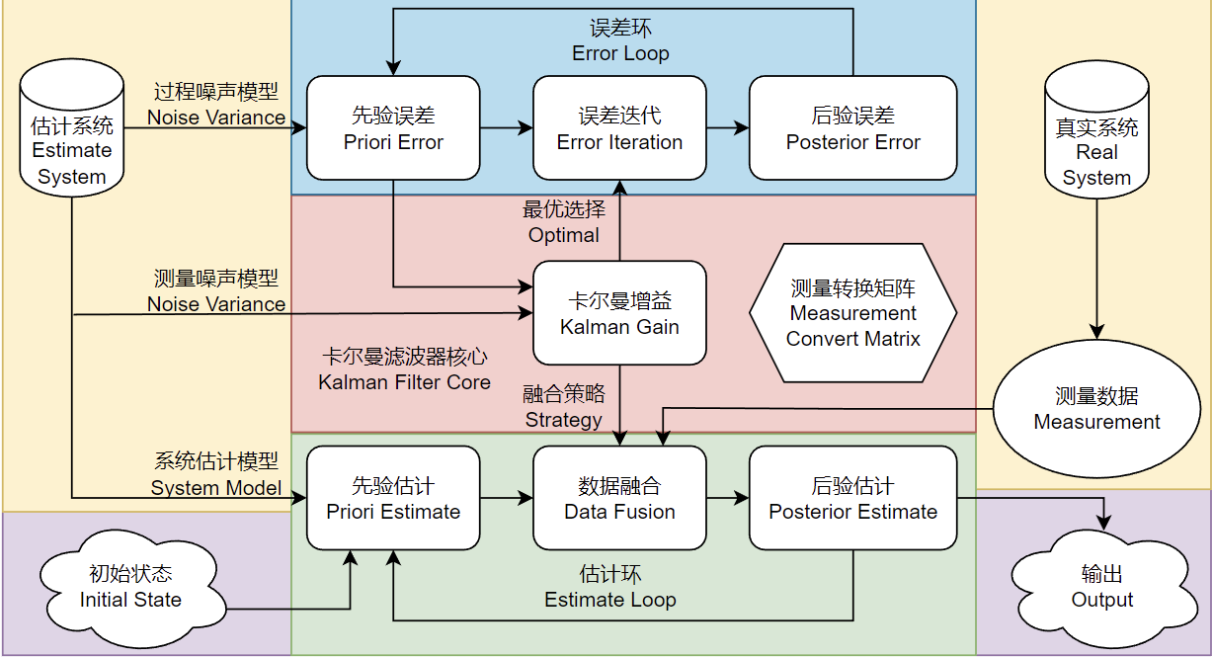
\includegraphics[scale=0.3]{figures/Kalman-Filter.png}
    \caption{Kalman Filter}
\end{figure}

\section{数据融合}

假设$\hat{x}^{-}_k$是模拟系统先验估计值,$\hat{x}^m_k$为测量系统测量到的$z_k$利用$z_k=H\hat{x}^m_k$反演得到理想实际值,也就是说这是测量值,假设系数矩阵$G$使得

\begin{equation}
    \hat{x}_k=(1-G)\hat{x}^{-}_k+G \hat{x}^m_k
\end{equation}

如果$G=0$,则后验估计偏向先验估计,$G=1$则偏向测量值。令$G=K_kH$,又有$z_k=H\hat{x}^{m}_k$,整理得到
\begin{equation}
    \begin{aligned}
        \hat{x}_k&=\hat{x}^{-}_k+G(\hat{x}^{m}_k-\hat{x}^{-}_k)=\hat{x}^{-}_k+K_kH(\hat{x}^{m}_k-\hat{x}^{-}_k)\\
        &=\hat{x}^{-}_k+K_k(z_k-H\hat{x}^{-}_k)\\
    \end{aligned}
    \label{eq1.3}
\end{equation}

我们的目标是估计\textbf{卡尔曼系数}使得后验估计的误差$e_k$最小。

\section{后验估计}

后验估计误差为$e_k=x_k-\hat{x}_k$,其中$x_k$是实际值,代入(\ref{eq1.3})
\begin{equation}
    \begin{aligned}
        e_k&=x_k-\left[\ \hat{x}^{-}_k+K_k(z_k-H\hat{x}^{-}_k)\ \right]\\
        &=x_k-\left[\ \hat{x}^{-}_k+K_k(H\hat{x}_k+\nu_k-H\hat{x}^{-}_k)\ \right]\\
        &=[I-K_kH]e^{-}_k+K_k\nu_k
    \end{aligned}
\end{equation}

其中$e^{-}_k$是先验误差,$\nu_k$是系统的测量误差,先验误差的定义如下

\begin{equation}
    \begin{aligned}
        e^{-}_k=x_k-\hat{x}^{-}_k&=(Ax_{k-1}+Bu_{k-1}+\omega_{k-1})-(A\hat{x}_{k-1}+Bu_{k-1})\\  
        &=A(x_{k-1}-\hat{x}_{k-1})+\omega_{k-1}\\
        &=Ae_{k-1}+\omega_{k-1}
    \end{aligned}
\end{equation}

在此基础上考虑到误差值中仅仅耦合了过程噪声和测量噪声,并且这两个噪声独立且服从各自的正态分布,我们可以说滤波器的先验误差和后验误差一定也符合正态分布,这个结论可以表达为下式
\begin{equation}
    \begin{aligned}
        & e_k\sim N(0,M_k),\ \ \ \ M_k=E[e_ke^T_k]\\
        & e^{-}_k\sim N(0,M^{-}_k),\ \ \ \ M^{-}_k=E[e^{-}_k(e^{-}_k)^T]\\
    \end{aligned}
\end{equation}

我们的目标是使的后验估计误差的方差最小,后验误差的协方差矩阵为
\begin{equation}
    \begin{aligned}
        E[ee^T]&=E\left[\ (I-K_kH)e^{-}_k+K_k\nu_k \ \right]\left[\ (I-K_kH)e^{-}_k+K_k\nu_k \ \right]^T\\
        &=E\left[\ (I-K_kH)e^{-}_k+K_k\nu_k \ \right]\left[\ (e^{-}_k)^T(I-K_kH)^T+\nu^T_kK^T_k \ \right]\\
        &=E[\ (I-K_kH)e^{-}_k\cdot (e^{-}_k)^T(I-K_kH)^T+K_k\nu_k\cdot (e^{-}_k)^T(I-K_kH)^T  \\
        &+(I-K_kH)e^{-}_k\cdot \nu^T_kK^T_k+K_k\nu_k\cdot  \nu^T_kK^T_k]\\
        &=E[(I-K_kH)e^{-}_k\cdot (e^{-}_k)^T(I-K_kH)^T]+E[K_k\nu_k\cdot (e^{-}_k)^T(I-K_kH)^T]\\
        &+E[(I-K_kH)e^{-}_k\cdot \nu^T_kK^T_k]+E[K_k\nu_k\cdot  \nu^T_kK^T_k]\\
    \end{aligned}
\end{equation}

由于测量误差$\nu_k$和先验误差$e^{-}_k$服从零均值的相互独立正态分布,因此中间两项为零,因此上式最终写成
\begin{equation}
\begin{aligned}
   M_k=E[ee^T]
    &=E[(I-K_kH)e^{-}_k\cdot (e^{-}_k)^T(I-K_kH)^T]+E[K_k\nu_k\cdot  \nu^T_kK^T_k]\\
    &=(I-K_kH)E[e^{-}_k\cdot (e^{-}_k)^T](I-K_kH)^T+K_kE[\nu_k\cdot  \nu^T_k]K^T_k\\
    &=(I-K_kH)M^{-}_k(I-K_kH)^T+K_kRK_k^T
\end{aligned}
\end{equation}

其中$R$是在本篇一开始就定义的$\nu_k$的协方差矩阵。根据协方差矩阵的性质,对角线就是后验估计误差的方差,因此我们取$M_k$的迹
\begin{equation}
    \begin{aligned}
        tr(M_k)&=tr[(I-K_kH)M^{-}_k(I-K_kH)^T]+tr[K_kRK_k^T]\\
        &=tr[M^{-}_k]-tr[K_kHM^{-}_k]-tr[M^{-}_kH^TK_k^T]\\
        &+tr[K_kHM^{-}_kH^TK^T_k]+tr[K_kRK_k^T]\\
        &==tr[M^{-}_k]-tr[K_kHM^{-}_k]-tr[K_kHM^{-}_k]\\
        &+tr[K_kHM^{-}_kH^TK^T_k]+tr[K_kRK_k^T]\\
    \end{aligned}
\end{equation}\footnote{这里用到对称矩阵迹的性质:$tr(A^T)=tr(A)$,$tr[(AB)^T]=tr[B^TA^T]$,$tr(A+B)=tr(A)+tr(B)$}

目标是选择$K_k$使的$tr(M_k)$最小化,由于方差是凸函数,所以极小值必然存在,根据极值存在的必要条件
\begin{equation}
    \frac{\partial\  tr(M_k)}{\partial K_k}=0\ \Rightarrow\ M_k^{-}H^T=K_k(HM^{-}_kH^T+R)
\end{equation}

因此我们可以给出\textbf{卡尔曼增益系数$K_k$}在最优估计下的表达式
\begin{framed}
    \begin{equation}
       K_k=\frac{M_k^{-}H^T}{HM^{-}_kH^T+R}
    \end{equation}
\end{framed}

将卡尔曼增益系数代回到数据融合方程里,就得到后验的表达
\begin{equation}
    \hat{x}_k=\hat{x}^{-}_k+\frac{M_k^{-}H^T}{HM^{-}_kH^T+R}(z_k-H\hat{x}^{-}_k)
\end{equation}

直观理解是:当测量误差$R$很大,估计趋于相信先验的估计,当$R$很小,则趋于相信仪器的测量。$R$源于仪器的固定属性,我们需要确定的是$M^{-}_k$
\begin{equation}
    \begin{aligned}
        M^{-}_k=E[(e^{-1}_k)(e^{-1}_k)^T]&=E[(Ae_{k-1}+\omega_{k-1})(Ae_{k-1}+\omega_{k-1})^T]\\
        &=E[Ae_{k-1}e^T_{k-1}A^T]+E[Ae_{k-1}\omega^T_{k-1}]+E[\omega_{k-1}A^Te^T_{k-1}]\\
        &+E[\omega_{k-1}\omega^T_{k-1}]\\
        & =AE[e_{k-1}e^T_{k-1}]A^T+E[\omega_{k-1}\omega^T_{k-1}]\\
        &=AM_{k-1}A^T+Q
    \end{aligned}
\end{equation}

这里$Q=E[\omega_{k-1}\omega^T_{k-1}]$过程误差的协方差矩阵,$M_{k-1}$为前面测得的后验误差协方差矩阵,这些都是前次计算得出来的数据,从这里也可以看出其实卡尔曼滤波是一种递归算法。

\section{算法}

由于数学推导很乱,我们在这里做一个总结
\begin{framed}
    \textbf{算法:(Kalman FIlter)}

    \begin{enumerate}[itemindent=2em]
        \item \textbf{预测} : 计算先验估计值$x^{-}_k$和先验误差的协方差矩阵$M^{-}_k$;
        \item \textbf{校正} : 计算卡尔曼增益系数$K_k$和后验估计$\hat{x}_k$;
        \item \textbf{额外更新} : 更新后验估计的误差协方差矩阵$M_k$,用来计算下一次的$M^{-}_{k+1}$;
    \end{enumerate}
\end{framed}

$k-1$次计算需要准备好的数据为$M_{k-1},Q,R$。